This chapter discusses the mathematical foundation for the numerical schemes which are presented in later chapters.
At the beginning of this chapter we repeat the basic definitions and notation for an analysis of partial differential equations as they are introduced for example in \cite[Introduction]{Evans1998}. Afterwards we introduce the finite element, as well as a discontinuous Galerkin method, for the latter we provide also a proof of its well-posedness. To prepare later calculations we end this chapter with some algebraic identities about the Hessian.

\section{ Preliminaries and Notation}
Let $\Omega \subset \R^d $ be an open, bounded area and $\partial \Omega$ its boundary.
\begin{definition}[Partial Differential Equation{\cite[Introduction]{Evans1998}}]
 A \emph{partial differential equation} (PDE) of order $k\in \N$ is an expression of the form
\begin{align}
	F(D^k u(x), D^{k-1}u(x), \dots, Du(x), u(x), x) = 0, \; (x \in \Omega)\label{eq:general PDE}
\end{align}
where $F:\R^{n^k} \times \R^{n^{k-1}} \times \dots \times \R^n \times \R \times \Omega \rightarrow \R $ is given and $u:\Omega \rightarrow \R$ is unknown.
\end{definition}
We focus in this thesis on second-order PDEs for our main PDE, namely the \emph{\MA equation} which we will introduce later is of second order. 
\\Beside the order there exist further properties to categorise PDEs:
\begin{definition}[Categories of PDEs{\cite[Introduction]{Evans1998}}] \label{def: categories of PDEs}
	Given functions  $f:\Omega \rightarrow \R$ and $a_{\alpha}:\Omega \rightarrow \R$ or $a_{\alpha}:\R^{n^{k-1}} \times \dots \times \R^n \times \R \times \Omega$ respectively, for $\alpha \in \N^{k}, |\alpha| \leq k$, a PDE of order $k$ is called
	\begin{enumerate}[(i)]
		\item \emph{linear} if it can be written in the form
		\[
			\sum_{|\alpha| \leq k} a_{\alpha} (x) D^{\alpha} u(x) = f(x).
		\] 
		
%		\item \emph{semilinear} if it can be written in the form
%		\[
%			\sum_{|\alpha| = k} a_{\alpha}(x) D^{\alpha} u + a_0(D^{k-1}u, \dots, Du, u, x)= f(x),
%		\]	
%		i.e. a semilinear PDE is nonlinear in the unknown function, but linear in all partial derivatives.
		
		\item \emph{quasilinear} if it can be written in the form
		\[
			\sum_{|\alpha| = k} a_{\alpha}(D^{k-1}u, \dots, Du, u, x) D^{\alpha} u + a_0(D^{k-1}u, Du, u, x)= f(x),
		\]	
		i.e. a quasilinear PDE is nonlinear in (at least) one lower derivate, but linear in the highest order derivates.
		
		\item \emph{fully nonlinear} if it depends nonlinearly upon the highest order derivatives.
	\end{enumerate}
\end{definition}
The standard example for linear PDEs is the \emph{Poisson equation} $-\triangle u = f$.
% a semilinear PDE is for example the \emph{nonlinear Poisson equation} $-\triangle u = f(u)$.
A well-known example for quasilinear PDEs are equations of the type $\nabla \cdot (A(u) \nabla u) = f$, where $A: \R^d \rightarrow \R^{d \times d}  $. The \MA equation $\mydet {D^2 u} = f$ is part of the last category, the nonlinear PDEs. 

Another important property to classify second-order PDEs is ellipticity. 
\begin{definition}[Elliptic PDE{, \cite[p.207]{FGN2013}}]
	A fully nonlinear second order PDE is called \emph{elliptic} if its operator satisfies
	\begin{align}
		F(A,p,z,x) \leq F(B,p,z,x) \label{eq: ellipitic PDE}
	\end{align}
for all $x \in \Omega, z \in \R, p \in \R^d$ and $A,B \in \R^{d \times d}_{sym}$  with $A-B$ positive semidefinite.

%This notion is a natural extension of the ellipticity concept for first order PDEs. Interpreting a first order PDE operator as a function depending on $D^2u, Du, u, x$, \eqref{eq: ellipitic PDE} characterises an elliptic PDE.
\end{definition}

Searching for a function $u:\Omega \rightarrow \R$ with 
\begin{align}
u=g \text{ on } \partial \Omega \label{eq: boundary}
\end{align}
for some $g:\partial \Omega \rightarrow \R$ is called a \emph{Dirichlet-boundary problem}. The function $u:\Omega \rightarrow \R$ fulfilling \eqref{eq:general PDE} and \eqref{eq: boundary} is called a classical solution of the problem. 

There are problems such that no classical solution exists. A PDE of order $k$ requires its classical solution to be at least $k$ times differentiable, which is a very strong demand. To admit less regular solutions one aims for a weaker notion of a solution. Before doing this we specify some function spaces.

\begin{definition} [Function Spaces and Norms]\label{def: function spaces and norms}
Accordingly to the majority of the literature we refer by $W^{s,p}(\Omega)$ to the H\"older space, a set consisting of all $L^p(\Omega)$ functions whose distributional derivates up to order $s$ are contained in $L^ p(\Omega)$.
In the special case $p=2$ they are referred to as Sobolev spaces $H^s(\Omega):=W^{s,2}(\Omega)$. An additional subscript $0$ denotes the set where all functions are zero at the boundary, i.e. $H^s_0 :=\{f \in H^s(\Omega); f(x)=0 \; \forall x \in \partial \Omega\}$.

The corresponding function space norms are defined by
\[
	\norm f _{W^{s,p}(\Omega)} = \left( \sum_{|\alpha| \leq s} \norm{D^\alpha f}^p_{L^p(\Omega)}\right)^{\frac 1 p }, \text{   especially } \norm f _{H^{s}(\Omega)}=\left( \sum_{|\alpha| \leq s} \norm{D^\alpha f}^2_{L^2(\Omega)}\right)^{\frac 1 2 }
\]
and the $H^s$ semi-norms
\[ 
 	|f|_{H^{s}(\Omega)}=\left( \sum_{|\alpha| = s} \norm{D^\alpha f}^2_{L^2(\Omega)}\right)^{\frac 1 2 }.
\]
%If not stated otherwise $\bilin f g$ always refer to the standard $L^2$ scalar product 
%\[
%	\bilinLTwo{f}{g} = \myInt_{\Omega } f g.
%\]
For a normed function space $X$ we denote its dual by $X'$ and by $\bilin{\cdot}{\cdot}$ the pairing between $X$ and $X'$.

\end{definition}
By this definition it is clear that the $H^0$ norm and the $L^2$ norm conincide. 

Let $T$ be the triangle in $\Omega$ spanned by the points $v_0, v_1, v_2$. We also write 
\[
	T= \langle v_0, v_1, v_2 \rangle := \{\beta_0 v_0+ \beta_1 v_1 +\beta_2 v_2; \sum_{i=0}^2 \beta_i =1, \beta_i \geq 0, i= 0,1,2\}.
\]
We define the \emph{diameter} $diam(T)$ of a triangle $T$ as the diameter of the smallest circle containing $T$.

To discretise our domain $\Omega$ we subdivide it into simplices, more precisely we divide it into triangles.
\begin{definition}[Triangulation, {\cite[Definition 5.1]{Braess2003}}]
	We call a finite partition of $\Omega$ into triangles $\{T_1, \dots, T_n\}$ a feasible \emph{triangulation} $\mathcal{T}$, such that
	\begin{enumerate}[(i)]
		\item	$\overline \Omega = \bigcup_{T \in \triang} T$
		\item If $T_i \cap T_j$ is a point for $i \neq j$ , it is a vertex of both $T_i$ and $T_j$.
		\item If $T_i \cap T_j$ is more than one point for $i \neq j$, it is an edge of both $T_i$ and $T_j$.
	\end{enumerate}
	Let $h$ denote the maximal diameter $h:= \operatorname{max}\limits_{T\in \mathcal T} diam(T)$ in the triangulation $\mathcal T$, we then also refer to $\mathcal{T}$ by $\triang$. We call a triangulation \emph{regular} if every element is congruent.
\end{definition}
Note that this definition requires $\Omega$ to be a polygonal domain. However, there are extensions to domains with curved boundaries: In those triangles lying at the boundary are replaced by \quoting{triangles} which have curved sides. 

\begin{figure}[H]
\usetikzlibrary{calc}

		\begin{center}
		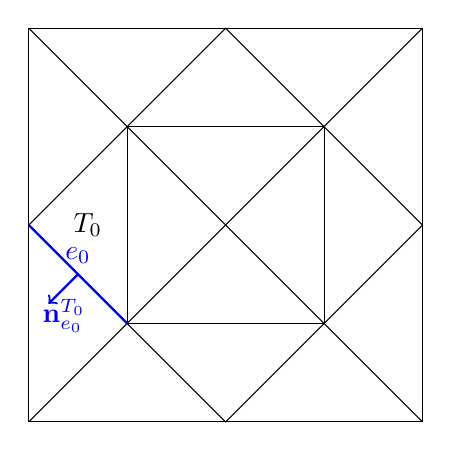
\begin{tikzpicture}[scale = 5]
%define coordinates
			\coordinate (vEins) at (0,0) ;
			\coordinate (vZwei) at (0:4cm);
			\coordinate (vDrei) at (90:4cm);

%draw square
			\draw (0,0) -- (1,0) -- (1,1) -- (0,1) -- cycle; 

%draw diagonals
			\draw (0,0) -- (1,1);
			\draw (1,0) -- (0,1);

			\draw (0.5,0) -- (1,0.5) -- (0.5,1)-- (0,0.5) --cycle; 

			\draw(0.25,0.25) -- (0.75,0.25) -- (0.75,0.75)-- (0.25,0.75) --cycle; 

			\draw node at (0.15,0.5) {$T_0$};

			\draw[color=blue, thick] (0.25,0.25)-- node[above]{\blue{$e_0$}} (0,0.5);
			\coordinate (vMiddle) ($(0.25,0.25)!0.5!(0,0.5)$);
			
			\draw[color=blue, thick, ->] ($(0.25,0.25)!0.5!(0,0.5)$) -- node[right=0.3, below=0.1]{\blue{$\mathbf n_{e_0}^{ T_0}$}} ($ ($(0.25,0.25)!0.5!(0,0.5)$) - (0.075,0.075)$);

		\end{tikzpicture}
		\end{center}

\caption{A regular triangulation of the unitsquare}
 \label{fig: triangulation}
\end{figure}

Figure \ref{fig: triangulation} shows a triangulation of the unit square. Since the edges uniquely define a triangulation of $\Omega$, we later also use the terms grid and mesh to refer to a subdivision into triangles.
An edge $e$ is called an interior edge if $e=T^+ \cap T^-$ holds for some $T^+,T^- \in \triang$, whereas it is called a boundary edge if $e \subset \partial \Omega$.
We divide the edges $\edges$ into the subsets $\edgesi$ and $\edgesb$ containing all interior edges and boundary edges, respectively. 
When we refer to a normal of an edge we always refer to an outward directed normal of one of the adjacent triangles. If it is not clear from the context to which triangle is referred we clarify that with a superscript.

On this basis we define some piecewise spaces.
\begin{definition}[Broken Spaces]
We define function spaces associated to a triangulation $\triang$ by
\begin{align*}
	H^s(\Omega;\triang) &:= \{f \in L^2(\Omega); f|_T \in H^s(T) \text{ for every } T \in \triang\}, \\
	\text{and }
	W^{s,p}(\Omega;\triang) &:= \{f \in L^p(\Omega); f|_T \in H^s(T) \text{ for every } T \in \triang\}.
\end{align*}	
\end{definition}

\begin{definition}[Piecewise Polynomial Spaces] \label{def: piecewise polySpace}
	Further we denote the finite-dimensional space of piecewise polynomials by
\[	
	\mathcal P^k_h = \{ f \in L^2(\Omega); f \arrowvert_T \textnormal{ is a polynomial of (total) degree } \leq k \textnormal{ for every } T \in \triang\}.
\]
\end{definition}

For later analysis we need the approximation properties of $\mathcal P_h^k$ proven in \cite[Chapter 4]{BS2002}, as well as standard trace and inverse estimates as proven in \cite[Section 1.6 and Section 4.5]{BS2002}.
\begin{lemma}[Approximation properties of $\mathcal P_h^k${,\cite[Theorem(4.4.20)]{BS2002}}]  \label{la: approximation properties}
Let $s,m \in \N$ with $0 \leq m \leq s\leq k+1$. Then for any $u \in H^s(\Omega)$, there exists $v_h \in \mathcal P^k_h$ such that 
\[
	\left( \sum_{T \in \triang} \norm{u-v_h}^2_{H^m(T)} \right)^{\frac 1 2} \leq C h^{s-m} \norm{u}_{H^{s}(\Omega)},
\]
where $C$ is a constant depending only on the mesh, but not in $h$ or $u$.
\end{lemma}
\begin{lemma}[Trace estimate{,\cite[Theorem(1.6.6)]{BS2002}}]\label{la: trace estimate}
	Given any quasi-uniform trianguliaton $\triang$, there holds for $ v \in H^1(\Omega;\triang)$
	\begin{align*}
	%	\norm{v}_{L2 (\partial T)}^2 \leq C\left(\frac 1 {h_T} \norm{v}_{L2(T)}^2  + h_T \norm{\nabla v}_{L2(T)}^2\right) \qquad \forall v \in H^1(T).
	\sum_{e \in \edges} \LTwonormE{v}^2 
		\leq C_1
		 \sum_{T \in \triang} \LTwonormT{v}^2 \HOnenormT{v}^2
	\leq 
		C_2 \sum_{T \in \triang} \left(\frac 1 {h} \LTwonormT{v}^2  + h \HOnenormT{v}^2\right).
	\end{align*}
	 where $C_1,C_2$ are positive constants depending only on the mesh but not on $v$.
\end{lemma}
Note that the second inequality follows from the identity $\sqrt{a} \sqrt{b} \leq \varepsilon a + \frac 1 \varepsilon b$ for arbitrary $a,b \in \R^+$ and $\varepsilon \geq 0$. This identity can be easily verified taking the root of the inequality $ab \leq \varepsilon^2 a^2 + 2ab + {\frac 1 \varepsilon}^2b^2 = \left( \varepsilon a + \frac 1 \varepsilon b\right)^2$.

\begin{lemma}[Inverse Estimate{, \cite[Lemma 2.4]{BGN+2011}}]\label{la: inverse estimate}
	For any piecewise polynomial $v \in \mathcal P_h^k$ there holds
	\[
	\norm v_{H^m(T)} \leq C h^{s-m} \norm v_{H^s(T)} \qquad \forall T \in \triang
	\]
\end{lemma}

To formulate a method capable of handling discontinuities along triangle edges we introduce edge operators.   
\begin{definition}[Edge Operators] \label{def: edge operators}
We denote the \emph{normal jump} of  a piecewise smooth function $u_h:\Omega \rightarrow \R$ across an edge $e \in \edges$ by
\begin{align*}
	\jump {u_h}&:= 
	\begin{cases}
		u_h^+  \mathbf n^+ + u_h^- \mathbf n^-  &\text{ if } \partial T^+ \cap \partial T^- = e \text{ for some }T^+,T^- \in \triang, \\
		u_h \mathbf n 	 &\text{ if } \partial T \cap \partial \Omega = e \text{ for some } T \in \triang,
	\end{cases}	
\end{align*}
where $n^\pm$ are the normals with respect to $T^\pm$ and  $u_h^\pm(x) := \lim_{\varepsilon \rightarrow 0} u_h(x-n^\pm \varepsilon)$.
Likewise we define the normal jump of a piecewise smooth function $u_h:\Omega \rightarrow \R^2$ across an edge $e \in \edges$ by
\begin{align*}
	\jump {u_h}&:= 
	\begin{cases}
		u_h^+ \cdot \mathbf n^+ + u_h^-\cdot  \mathbf n^-  &\text{ if } \partial T^+ \cap \partial T^- = e \text{ for some }T^+,T^- \in \triang,\\
		u_h\cdot \mathbf n 	 &\text{ if } \partial T \cap \partial \Omega = e \text{ for }T\in \triang.
	\end{cases}	
\end{align*}
Here $\cdot$ denotes the scalar product.
Note that the jump of a scalar is a vector, whereas the jump of a vector is a scalar.

The \emph{average} of a piecewise smooth function $u_h:\Omega \rightarrow X$ for every $X$ across an edge $e \in \edges$ is defined by
\begin{align*}
	\average {u_h} &:= 
	\begin{cases}
	\frac 1 2 \left(u_h^+ + u_h^-\right) &\text{ if } \partial T^+ \cap \partial T^- = e \text{ for some }T^+,T^- \in \triang, \\
	 u_h &\text{ if } \partial T \cap \partial \Omega = e \text{ for }T\in \triang.
	\end{cases}
\end{align*}
\end{definition}

We end this section with the note that we use a subscript $h$ to indicate a piecewise evaluation or interpretation.  Subsequently differential operators with a subscript $h$ imply that differentiations were carried out seperately on every triangle, for example the piecewise gradient is defined by $\nabla_h f |_T = \nabla f |_T \; \forall T \in \triang$. 



\section{Finite Element Method}
Before we discuss numerical schemes for the \MA equation we shortly recall how a finite element method works, for a deeper insight in finite element methods we recommend \cite{Braess2003, BS2002}. Since the finite element method bases on a variational formulation we introduce the method talking about the well-known example of the generalised Poisson equation. 

%\subsection{The Poisson Problem}

\begin{definition}[generalised Poisson Problem] \label{def: General Poisson Problem}
The \emph{generalised Poisson Problem} is finding a function $u:\Omega \rightarrow \R$ such that 
\begin{align}
	-\nabla \cdot (A \nabla u) = f \qquad &\text{ in }\Omega \label{eq: poisson eq} \\
	u = g \qquad &\text{ on } \partial \Omega    \label{eq: poisson bc}
\end{align}
for $ A:\Omega^d \rightarrow \R^{d \times d}$ symmetric and functions $f,g:\Omega \rightarrow \R $. 
Because of the physical context of this PDE the matrix $A$ is also referred to as \emph{diffusion matrix}.
\end{definition}

We are now able to set up a \emph{weak formulation} of the generalised Poisson problem based on variational principles, this formulation is the key element for deriving a finite element method.

Due to the main theorem of variational analysis every classical solution to \eqref{eq: poisson eq} is fulfils 
\begin{align}
	-\myIntX \Omega {\varphi \nabla \cdot (A \nabla u)}=
	 \myIntX \Omega {\varphi f} \qquad \forall \varphi \in C^\infty(\Omega), \label{eq: variational form}
\end{align}
and vice versa.
Integration by parts yields to
\begin{align*}
	\myIntX \Omega {\nabla \varphi  \cdot A\nabla u}
		-\myIntS  {\partial \Omega} { \varphi (A\nabla u) \mathbf{n} }
	= \myIntX  \Omega { \varphi f } \qquad \forall \varphi \in C^\infty(\Omega). %\label{eq: FE integration by parts}
\end{align*}
The last statement can be reformulated to the so called variational form 
\begin{align}
a(\varphi,u)  = b(\varphi) \qquad \forall \varphi \in C^\infty(\Omega). \label{eq: variational formulation}
\end{align}
with the bilinear form $a:C^\infty(\Omega) \times X \rightarrow \R$
\begin{align*}
a(\varphi,u) = \myIntX  \Omega { \nabla \varphi  \cdot A\nabla u }
	 -\myIntS  {\partial \Omega} { \varphi (A\nabla u) \mathbf{n}}
\end{align*}
where $X$ is a function space we define in a moment and the functional $b:C^\infty(\Omega) \rightarrow \R$
\begin{align*}
 b(\varphi)  = \myIntX  \Omega { \varphi f}.
\end{align*}


\begin{definition}[Weak Solution]
	Functions satisfying \eqref{eq: variational formulation} are called \emph{weak solutions} of \eqref{eq: poisson eq}.
\end{definition}
Note that due to the lack of regularity weak solutions may not be restricted to the boundary of $\Omega$. However one can reformulate boundary conditions for weak solution with trace operators \cite[Section 5.5]{Evans1998}.

The generalised Poisson problem is well-posed in the sense that it has a unique weak solution if $A$ is positive definite and $f\in L^2(\Omega)$. This is mainly due to the ellipticity of the PDE (and as a consequence thereof the ellipticity of $a$). Thus, it is possible to apply the Lax-Milgram theorem and a maximum principle. For an analysis we refer the interested reader to \cite[Chapter~6]{Evans1998}.

On the left-hand side in the weak notation only first derivatives of $u$ appear, hence \eqref{eq: variational formulation} is also applicable for functions $u$ which are not twice differentiable. It turns out that the previously defined Sobolev spaces are well-suited candidates for the space $X$ containing weak solutions \cite[Chapter 1]{BS2002}. Therefore we search for the solution of the infinite-dimensional problem: Find $u\in H^1(\Omega)$ such that  $a(\varphi,u)  = b(\varphi) \;\forall \varphi \in C^\infty(\Omega)$ holds. \\% $\forall \varphi \in C^\infty(\Omega)$.
The main idea of the finite element method is to approximate the two function spaces, namely the spaces $H^1(\Omega)$ and $C^\infty(\Omega)$ containing $\varphi$ and $u$, respectively by finite dimensional spaces $W_h$ and $V_h$. For those spaces should hold a analogous equation as we have in the variational form stated in \eqref{eq: variational formulation}.\\
The finite space $W_h$ is called \emph{test space} and its elements are called \emph{test functions}. $V_h$ is referred to as \emph{ansatz} or \emph{trial space}, the contained functions accordingly \emph{ansatz} or \emph{trial functions}. To ensure the boundary condition \eqref{eq: poisson bc} we demand $u_h|_{\partial \Omega} = g$ for every $u_h \in V_h$.

Usually these limited function spaces are based on a discretisation of $\Omega$ and are only piecewise smooth. Consequently, we have to replace all operators appearing in $a$ by operators defined on $W_h \cup V_h$. We denote these discretised versions using the subscript $h$.

With these preliminaries we can define the finite element methods as searching for $u_h \in V_h$ such that 
\begin{align}
a_h(w_h,u_h) = b_h(w_h) \qquad \forall w_h \in W_h. \label{eq: FE variational formulation}
\end{align}
with the bilinearform  $a_h:W_h \times V_h \rightarrow \R$
\begin{align*}
a_h(w_h,u_h)  = \myIntX  \Omega { \nabla w_h  \cdot A\nabla u_h} -\myIntS  {\partial \Omega} { w_h (A\nabla u_h) \mathbf{n}}
\end{align*}
and the function $b:W_h \rightarrow \R$
\begin{align*}
b_h(w_h) = \myIntX  \Omega { w_h f}.
\end{align*}

This general proceeding is called a \emph{Galerkin approach}. Choosing $W_h = V_h$ yields to the so-called \emph{Galerkin methods}, otherwise the methods are referred to as \emph{Petrov-Galerkin methods}.

To construct $u_h$ we first choose a basis $B_W$ of $W_h$ and a basis $B_V$ of $V_h$.
Since the left-hand side is linear in $w_h$ we only need to check the equations in \eqref{eq: FE variational formulation} for all $w_h \in B_W$. 
Furthermore we can express $u_h$ as the linear combination of basis functions, namely $\sum_{p \in B_V} \mathbf{c}_p \; p$ and hence, we can rewrite \eqref{eq: FE variational formulation} as a linear system of equations $M \mathbf{c} = \mathbf{b}$ where  $\mathbf{c}$ is the unknown coefficient vector of $u_h$ to the basis $B_V$.  The matrix $M$ sometimes is named the \emph{system} or \emph{stiffness matrix}.

Altogether a finite element method for the generalised Poisson equation is defined by the bilinearform $a$ and the functional $b$ together with the choice of $W_h$ and $V_h$. Its computations consist of the assembling process where the matrices $M$ and the right-hand side vector $b$ are computed and the solving process of the resulting linear system of equations.\\
The error made by restriction to finite elements is characterised by the following Lemma.
\begin{lemma}[C\'ea Lemma{, \cite[4.2]{Braess2003}}] \label{la: Ceas lemma}
	Let the bilinear form $a$ be $V$ elliptic with $H_0^m \subset V \subset H^m(\Omega) $, i.e. $0 < \alpha \leq C$ exist with
	\[
		a(u,u) \geq \alpha  \norm u ^2_V \text{ and } |a(v,u)| \leq C \norm u ^2_V \norm v ^2_V.
	\]
	Then for the solution $u_h$ of \eqref{eq: FE variational formulation}  holds
	\begin{align}
		\norm {u - u_h}_V \leq \frac C \alpha \inf\limits_{v_h \in V_h} \norm {u-v_h}_V.
	\end{align}
\end{lemma}
This result shows that the quality of the finite element solution depends on the one side on the problem parameters $\alpha$ and $C$, but on the other side particularly on the approximation properties of $V_h$. A typical choice for the function spaces $W_h$ and $V_h$ are piecewise polynomials spaces which have good approximation properties and are easy to handle.

\section{Discontinuous Galerkin} \label{sec: SIPG}
A recent idea is to to include discontinuous functions when choosing the test and ansatz spaces. This approach arose in the context of hyperbolic PDEs whose solutions eventually contain discontinuities, later it was also applied to elliptic PDEs \cite{ABC+2002}. Although the generalised Poisson problem is not hyperbolic and its solutions are continuous we use this example to explain the issues arising when the finite element spaces are extended to discontinuities. The crux is the handling of function evaluations along discontinuities. Note that for discontinuous ansatz spaces it is no longer true that they are subspaces of $H^1(\Omega)$ which contains the weak solution of the generalised Poisson problem. That implies that C\'eas Lemma \ref{la: Ceas lemma} is not valid. Elements which include ansatz space not contained in $H^1(\Omega)$ are also referred to as non-conforming elements.

%We recall our triangulation $\mathcal{T}_h$ of $\Omega$. 
If we modify the derivation of the bilinear form defining the finite element method we can develop bilinear forms defined on the function space $V_h = \mathcal P_h^k$ (cf. Definition \ref{def: piecewise polySpace}): Due to the fact that we have discontinuities only along edges we perform the integration by parts in \eqref{eq: variational form} piecewise on every triangle leading to
\begin{align}
	a(v, u) = & \sum_{T \in \triang} \myIntX T {\nabla v \cdot A \nabla u }
		- \sum_{T \in \triang} \myIntS  {\partial T} { v A \nabla u \cdot \mathbf n}.
\end{align}
Since two adjacent elements share the same edge only with opposite directed normal vectors we can rewrite the last term as
\begin{align*}
\sum\limits_{T \in \triang}\myIntS  {\partial T} { v A \nabla u \cdot \mathbf n }
= &\sum\limits_{e \in \edgesi}\myIntS e { \left( v^+ A^+ \nabla u^+ \cdot \mathbf n^+ + v^- A^- \nabla u^- \cdot \mathbf n^- \right)} \\
& + \sum\limits_{e \in \edgesb}\myIntS e { v A \nabla u \cdot \mathbf n},
\end{align*}
where $h^\pm $ is $h$ evaluated in one of the two adjacent elements $T^\pm$ with $T^+ \cap T^- = e$. With the identity $\mathbf n^- = -\mathbf n^+$ we can extend
\begin{align*}
	&v^+ A^+ \nabla u^+ \cdot \mathbf n^+ + v^- A^- \nabla u^- \cdot \mathbf n^- \\
		= & \phantom{+} v^+ A^+ \nabla u^+ \cdot \mathbf n^+ 
		     + \frac 1 2  v^+ A^- \nabla u^- \cdot \mathbf n^- + \frac 1 2 v^+ A^- \nabla u^- \cdot \mathbf n^+ \\
		& + \frac 1 2  v^- A^+ \nabla u^+ \cdot \mathbf n^+ + \frac 1 2 v^- A^+ \nabla u^+ \cdot \mathbf n^-
		   + v^- A^- \nabla u^- \cdot \mathbf n^-.
\end{align*}
Splitting up first and last term, we find this equals to
\begin{align*}
		 & \phantom{+} \frac 1 2 v^+ A^+ \nabla u^+ \cdot \mathbf n^+ 
		     + \frac 1 2  v^+ A^- \nabla u^- \cdot \mathbf n^- + \frac 1 2  v^- A^+ \nabla u^+ \cdot \mathbf n^+ + \frac 1 2 v^- A^- \nabla u^- \cdot \mathbf n^- \\
		& + \frac 1 2  v^+ A^+ \nabla u^+ \cdot \mathbf n^+  + \frac 1 2 v^+ A^- \nabla u^- \cdot \mathbf n^+ +\frac 1 2 v^- A^+ \nabla u^+ \cdot \mathbf n^- + \frac 1 2 v^- A^- \nabla u^- \cdot \mathbf n^-\\
		    	  = & \phantom{+} \frac 1 2 \left(v^+ + v^- \right) \left(A^+ \nabla u^+ \cdot \mathbf n^+ + A^- \nabla u^- \cdot \mathbf n^- \right) \\
  &+  v^+ \frac 1 2  \left(A^+ \nabla u^+ + A^- \nabla u^-\right) \cdot \mathbf n^+ + v^- \frac 1 2 \left(A^+ \nabla u^+ + A^- \nabla u^-\right) \cdot \mathbf n^- \\
  = &  \jump {\average v  A \nabla u}+ \jump {v \average{ A \nabla u}}.
\end{align*}
Therefore the weak formulation can be written as $a(v,v) = l(v)$ with 
\begin{align*}
  a(v, u) = & \sum\limits_{T \in \triang} \myIntX  T { \nabla v \cdot A \nabla u} \\
	& - \sum\limits_{e \in \edgesi}\myIntS {e} {\left( \jump {\average v A \nabla u} + \jump {v \average{ A \nabla u}} \right)}\\
& - \sum\limits_{e \in \edgesb}\myIntS {e} {v A \nabla u \cdot \mathbf n}
\end{align*}
and
\[
l(v) = \sum_{T \in \triang} \myIntX  T { v f}.
\]
Due to the smoothness of the exact solution $u$ we neglect the jump in $A \nabla u$, i.e. $\jump A \nabla u =0$, and find
\begin{align*}
 a(v, u) = & \sum\limits_{T \in \triang} \myIntX  T { \nabla v \cdot \left(A \nabla u\right)} %\\
	- \sum\limits_{e \in \edgesi} \myIntS e {\jump{ v \average{ A \nabla u}}} %\right)
	\\
& - \sum\limits_{e \in \edgesb}\myIntS e { v A \nabla u \cdot \mathbf n}.
\end{align*}

To get a symmetric system matrix we symmetrise our bilinear form $a$ by adding terms. 
The first term we add is  $- \sum\limits_{e \in \edgesi}\myIntS e { \jump{ u \average{ A \nabla v}}}$ which equals zero when evaluating the integral for a smooth $v$. Hence it will vanish for the solution of the generalised Poisson problem. The second term required to achieve symmetry is  $-\sum\limits_{e \in \edgesb}\myIntS e { u A \nabla v \cdot \mathbf n}$. Since the Dirichlet boundary condition gives us solution values at the boundary this term equals $\sum\limits_{e \in \edgesb}\myIntS e { g A \nabla v \cdot \mathbf n}$. Thus, we simply add it to both to the bilinear form and to the right-hand side functional.
\begin{align}
 a_S(v, u) = &\sum\limits_{T \in \triang} \myIntX  T { \nabla v \cdot A \nabla u} \nonumber \\
  &-\sum\limits_{e \in \edgesi}\myIntS e { \jump {v \average{A \nabla u} }}
 - \sum\limits_{e \in \edgesi}\myIntS e { \jump{ u \average{ A \nabla v}}} \nonumber\\ 
 & - \sum\limits_{e \in \edgesb}\myIntS e { v A \nabla u \cdot \mathbf n} 
    - \sum\limits_{e \in \edgesb}\myIntS e { u A \nabla v \cdot \mathbf n} \nonumber
\end{align}
and 
\begin{align}
	l(v) =& \sum\limits_{T \in \triang} \myIntX  T { v f}
		 -\sum\limits_{e \in \edgesb}\myIntS e { g A \nabla v \cdot \mathbf n}.
\end{align} 
Since we defined the jump and average also on boundary edges (cf. Definition \ref{def: edge operators}) we can shorten the term to 
\begin{align}
a_S(v, u)= &\sum\limits_{T \in \triang} \myIntX  T { \nabla v \cdot A \nabla u} \nonumber \\  &-\sum\limits_{e \in \edges}\myIntS e { \jump {v \average{A \nabla u} }}
 - \sum\limits_{e \in \edges}\myIntS e { \jump{ u \average{ A \nabla v}}}. \label{eq:inner product SIPG}
\end{align}

%and $f$
%\begin{align}
%	f_S(v,v) = && \sum\limits_{T \in \triang} \myIntX  T { v f \\
%	 				&+ &\sum\limits_{e \in \edgesb}\myIntS e { v \cof(D^2 w) \nabla u \cdot n \\
% &+ &\sum\limits_{e \in \edgesi}\myIntS e { u \llbracket \cof(D^2 w) \nabla v \cdot n\rrbracket \\
%	&-  &\sum\limits_{T \in \triang} \myIntX  T { u (\nabla \cdot \cof(D^2w)) \cdot \nabla v \\
%\end{align} 
We need to enforce continuity and compliance with the boundary conditions as our ansatz space is discontinuous and allows arbitrary boundary values. To do that, we penalise the jump across interior and boundary edges as described in  \cite[3.2.2.]{PPO+2000} by adding the two following terms to $a_S$ and $l$, respectively
\begin{align}
	J^\sigma(v, u) = \sum\limits_{e \in \edgesi} \myIntS e { \frac \sigma {|e|} \jump v \jump u}
		 \;\; \textnormal{ and } \;	\;
		 J^\sigma_0(v) = \sum\limits_{e \in \edgesb} \myIntS e {\frac \sigma {|e|} v g} . \label{eq: penalty term}
\end{align}

Thus, we end up with the problem of finding $v \in V_h$ such that
\begin{align}
	a_h^{DG}(v, u) = l^{DG}_h (v) \qquad \forall v \in V \label{eq: DG system}
\end{align}
where
\[ 	
	a_h^{DG} (v, u) := a_S(v,u) + J^\sigma(v,u) \text{ and } l_h^{DG}(v) := l(v) + J^\sigma_0(v).
\]

%The authors of \cite{PPO+2000} suggest to choose the penalty term $\sigma$ as $10 k^2$ and undergird that 

Just like in the finite element method we can derive a linear system of equations $M \mathbf{u} = \mathbf{l}$ with $M$ sparse and $\mathbf{u}$ representing the coefficient vector of $u_h$ with respect to the basis $B_V$.
This particular discontinuous Galerkin method is called \emph{Symmetric Interior Penalty Galerkin method} (SIPG).

\section{Well-posedness of the SIPG Method}

In this section we want to prove the derived SIPG method is well-posed.
In this section we want to prove th derived SIPG method is well-posed. The norm to carry out an analysis easily is the discrete energy norm.
Let $V$ be $H^1(\Omega; \triang)$ and the bilinear form $\bilin \cdot \cdot_A:V \times V$ be given by
\begin{align}
	\bilin \varphi v _ A =  \sum_{T \in \triang} \int_T \nabla \varphi \cdot A \nabla v
\end{align}
\begin{definition}[Energy Norm] \label{def: energy norm}
		The mesh-dependent energy norm for a function $v \in V$ is defined by
		\[
			\eNorm v ^2 := \bilinA v v + \frac 1 \sigma \sum_{e \in \edges} |e|\LTwonormE{\average{A \nabla v}} + 2  \sigma \sum_{e \in \edges} \frac 1 {|e|}\LTwonormE{\jump{\nabla v}}.
		\]
\end{definition}
\todo{$\Omega,\triang$ erklaren}

Note that through this section $C$ denotes a generic positive constant independent of $h$ that may take different values in each equation.

At first, we show the following statement
\begin{lemma}[Boundedness of the SIPG method]\label{la: SIPG continuous}
	For the SIPG method holds
	\[
		|a_S(\varphi, v) + J^\sigma(\varphi,v)| \leq \eNorm{\varphi} \eNorm{v} \qquad \forall \varphi,v \in V_h
	\]
\end{lemma}
\begin{proof}
Let us consider the terms of \eqref{eq:inner product SIPG} separately.
For the first term we have by the Cauchy-Schwarz inequality
\begin{align}
	|\sum\limits_{T \in \triang} \int_T \nabla \varphi \cdot A \nabla v| =& |\bilinA {\nabla \varphi} {\nabla v} | \leq \left( {\bilinA {\nabla \varphi} {\nabla \varphi}}\right)^{\frac 1 2 } \left( {\bilinA {\nabla v}{\nabla v}}\right)^{\frac 1 2 }. \label{eq: CS estimate 0}
\end{align}
Considering the sum of the second and the fourth term we find using Cauchy-Schwarz and using also the discrete Cauchy-Schwarz inequality
\begin{align}
	|\sum\limits_{e \in \edges}\int_{e} \jump {\varphi \average{A \nabla v} }| &\leq
	\sum\limits_{e \in \edges}  \LTwonormE{\jump {\varphi}} \LTwonormE {\average{A \nabla v}} \nonumber \\
	& \leq
		\left( \sum\limits_{e \in \edges} \frac {\sigma}{|e|} \LTwonormE{\jump {\varphi}}^2 \right)^{\frac 1 2}
		\left( \sum\limits_{e \in \edges} \frac {|e|} \sigma \LTwonormE{\average{A \nabla v}}^2 \right)^{\frac 1 2} \label{eq: CS estimate}
\end{align}
Since the third and the last term in \eqref{eq:inner product SIPG} are the symmetrising terms, we analogously have for their sum
\begin{align}
\sum\limits_{e \in \edges}\int_{e} \frac 1 {|e|}\jump {v \average{A \nabla \varphi} } \leq&
			\left( \sum\limits_{e \in \edges} \frac {\sigma}{|e|}\LTwonormE{\jump {v}}^2 \right)^{\frac 1 2}
			\left( \sum\limits_{e \in \edges} \frac {|e|} \sigma \LTwonormE{\average{A \nabla \varphi}}^2 \right)^{\frac 1 2}.\label{eq: CS estimate2}
\end{align}
Now only the last term of \ref{eq:inner product SIPG} needs to be estimated. Again we apply at first the Cauchy-Schwarz inequality and then the discrete Cauchy-Schwarz inequality:
\begin{align}
\singleNorm {\sum_{e \in \edgesi} \frac \sigma {|e|} \int_e \jump \varphi \jump v }
\leq& \sum_{e \in \edgesi} \frac \sigma  {|e|} \int_e \singleNorm {\jump \varphi \jump v }
\leq \left( \sum\limits_{e \in \edges} \frac \sigma{|e|} \LTwonormE{\jump{\varphi}}^2 \right)^{\frac 1 2} \left( \sum\limits_{e \in \edges} \frac \sigma {|e|} \LTwonormE{\jump{v}}^2 \right)^{\frac 1 2} \label{eq: CS estimate3}
\end{align}
Adding \eqref{eq: CS estimate 0}, \eqref{eq: CS estimate}, \eqref{eq: CS estimate2} and \eqref{eq: CS estimate3} we find using the discrete Schwarz inequality once more
\begin{align}
	|a_S(\varphi,v)| \leq& 
		\left( {\bilinA {\nabla \varphi} {\nabla \varphi}}\right)^{\frac 1 2 } \left( {\bilinA {\nabla v}{\nabla v}}\right)^{\frac 1 2 } \nonumber\\
	& +\left( \sum\limits_{e \in \edges}\frac {\sigma}{|e|}\LTwonormE{\jump {\varphi}}^2 \right)^{\frac 1 2}
			\left( \sum\limits_{e \in \edges} \frac {|e|} \sigma \LTwonormE{\average{A \nabla v}}^2 \right)^{\frac 1 2} \nonumber\\
	& +	\left( \sum\limits_{e \in \edges} \frac {\sigma} {|e|}\LTwonormE{\jump {v}}^2 \right)^{\frac 1 2}
				\left( \sum\limits_{e \in \edges} \frac {|e|} \sigma \LTwonormE{\average{A \nabla \varphi}}^2 \right)^{\frac 1 2}\nonumber \\
	& + \left( \sum\limits_{e \in \edges} \frac \sigma{|e|} \LTwonormE{\jump{\varphi}}^2 \right)^{\frac 1 2} \left( \sum\limits_{e \in \edges} \frac \sigma {|e|} \LTwonormE{\jump{v}}^2 \right)^{\frac 1 2} \nonumber \\
	\leq& 
	\left( 
		\bilinA {\nabla \varphi} {\nabla \varphi}+2\sum\limits_{e \in \edges} \frac {\sigma} {|e|}\LTwonormE{\jump {\varphi}}^2+ \sum\limits_{e \in \edges} \frac {|e|} \sigma \LTwonormE{\average{A \nabla \varphi}}^2
	\right)^{\frac 1 2} \nonumber \\
	&\times
		\left( 
			\bilinA {\nabla v} {\nabla v}+2\sum\limits_{e \in \edges} \frac {\sigma}{|e|}\LTwonormE{\jump {v}}^2+ \sum\limits_{e \in \edges} \frac {|e|} \sigma \LTwonormE{\average{A \nabla v}}^2
		\right) ^{\frac 1 2} \\
		= & \eNorm \varphi \eNorm v 
\end{align}
\end{proof}

The next step in our analysis considers the stability of the SIPG method. To do we first need to define a norm measuring ???\todo{yeah what} 
\begin{definition}[$H^{-1}$ Semi-norm] \label{def: h-1 seminorm}
	The semi-norm is given by 
	\[
		\HMinusOneDnorm r ^2 := \sup_{0 \neq w \in V_h} \frac {{\bilin r w } } {\eNorm{w}}.
	\]
\end{definition}
Before we can start we need to define yet another mesh-dependent energy norm which later simplify the proof that the left-hand side's bilinear form of the SIPG method is coercive.
\begin{definition}[Energy Norm]\label{def: energy norm2}
The mesh-dependent discrete energy norm $\eNormTwo \cdot $ is defined by
\[
		\eNormTwo v^2 :=  \bilinA v v +  \sigma \sum_{e \in \edges} \frac 1 {|e|}\LTwonormE{\jump{\nabla v}}.
\]
\end{definition}
Calling this norm also an energy norm is justified as both norms are equivalent on $V_h$.
\begin{lemma}[Equivalence of Energy Norms in $V_h$]
	For any $w \in V_h$ holds
		\[
			c \eNormTwo w \leq \eNorm w \leq C \eNormTwo w
		\]
		with positive Constants $c, C$ depending only on the mesh.
\end{lemma}
\begin{proof}
	By definition the inequality $c \eNormTwo w \leq \eNorm w$ is clear and holds for example for $c=1$. 
By the trace estimate we have
	\begin{align}
		\sum_{e \in \edges} \singleNorm e \LTwonormE{\average{A \nabla v}} 
		\leq C \sum_{T \in \triang} \left( \LTwonormT{\average{A \nabla v}} +\HOnenormT{\average{A \nabla v}}   \right).
	\end{align}
Recalling the definition of the average (cf. Definition \ref{def: edge operators}) it is clear we can further simplify to
		\begin{align}
			\sum_{e \in \edges} \singleNorm e \LTwonormE{\average{A \nabla v}} 
			\leq C \sum_{T \in \triang} \left( \LTwonormT{A \nabla v} +h^2 \HOnenormT{ A \nabla v}   \right).
		\end{align}

\end{proof}


\begin{theorem}[Stability]\label{thm: SIPG stability}
There holds for $a_h v :=a_S(\cdot, v)+J^\sigma(\cdot, v)$
	\begin{align*}
	 	\HMinusOneDnorm{a_h v} \leq \eNorm v \qquad \forall v \in V. %\label{eq: bilin continuity}
	 \end{align*}
	 Moreover, there exists a $\sigma^* > 0$ such that for $\sigma \leq \sigma^* $, the operator $a$ is invertible with 
	 \begin{align*}
	 	\eNorm {a_h^{-1} r} \leq C \HMinusOneDnorm r \qquad \forall r \in V_h %\label{eq: bilin stability}
	 \end{align*}
	 where $C$ is independent of $h$. 
\end{theorem}
\begin{proof}
	The first estimate follows directly from Lemma \ref{la: SIPG continuous} and the definition of the norm \ref{def: h-1 seminorm}. If are able to show $a$ is coercive on $V_h$, we may apply classical existence and uniqueness theory, namely the Lax-Milgram theorem and thus deduce the inversibilty in $V_h$.
	
	
	
	Since the diffusion matrix $A$ is positive definite it holds
	\begin{align}
		\int_\Omega \nabla w \cdot A \nabla w \geq \lambda \LTwonorm {\nabla w }^2  \label{eq: estimate pos def}
	\end{align}
	for a $\lambda >0$.
	It holds
	\begin{align}
		\bilin {a_h(v)} {v}  = \bilinA {\nabla v} {\nabla v} - 2 \sum\limits_{e \in \edges}\int_{e} \jump {v \average{A \nabla v} } + \sum_{e\in \edgesi} \frac \sigma {|e|} \int_e \jump v^2 .\label{eq: coerc first estimate}
	\end{align}
	We derived in \eqref{eq: CS estimate} the estimate 
	\begin{align}
\sum\limits_{e \in \edges}\int_{e} \jump {v \average{A \nabla v} }
 \leq		\left( \sum\limits_{e \in \edges} \frac {\sigma}{|e|} \LTwonormE{\jump {v}}^2 \right)^{\frac 1 2}
		\left( \sum\limits_{e \in \edges} \frac {|e|} \sigma \LTwonormE{\average{A \nabla v}}^2 \right)^{\frac 1 2} \label{eq: inter estimate}
 	\end{align}
	Taking the root of the trivial identity $ab \leq \varepsilon^2 a^2 + 2ab + {\frac 1 \varepsilon}^2b^2 = \left( \varepsilon a + \frac 1 \varepsilon b\right)^2$ yields the inequality $\sqrt{a} \sqrt{b} \leq \varepsilon a + \frac 1 \varepsilon b$ for arbitrary $a,b \in R$ and $\varepsilon \geq 0$. Thus, we can derive from \eqref{eq: inter estimate}
	\begin{align*}
		\sum\limits_{e \in \edges}\int_{e} \jump {v \average{A \nabla v} } \leq \frac 1 \varepsilon \sum\limits_{e \in \edges}\frac \sigma {|e|}\LTwonormE{\jump {v}}^2 
		+ \varepsilon  \sum\limits_{e \in \edges}  \frac {|e|} \sigma \LTwonormE{\average{A \nabla v}}^2
	\end{align*}
	Using this estimate in \eqref{eq: coerc first estimate} we can derive
	\begin{align*}
		a_h(v,v)  \geq&
		 \bilinA {\nabla v} {\nabla v} 
		 -	 2 \varepsilon  \sum\limits_{e \in \edges}  \frac {|e|} \sigma \LTwonormE{\average{A \nabla v}}^2
		 + \left(-\frac 1 \varepsilon +1\right) \sum_{e\in \edgesi}  \frac \sigma {|e|} \LTwonormE{\jump {v}}^2
	\end{align*}
	Subtracting $\alpha \eNorm v$ from both sides implies
	\begin{align}
	a_h(v,v) - \alpha  \eNorm v
	\geq& (1-\alpha) \bilinA {\nabla v} {\nabla v} 
	+ (-2 \varepsilon -\alpha) \sum\limits_{e \in \edges}  \frac {|e|} \sigma \LTwonormE{\average{A \nabla v}}^2 \nonumber\\
	 &+ \left(-\frac 1 \varepsilon +1-\alpha\right) \sum_{e\in \edgesi}  \frac \sigma {|e|} \LTwonormE{\jump {v}}^2.
	\end{align}
	If we can find values for $\sigma$ and $\varepsilon$ such that the right-hand side is positive we proved the coercivity. To further simplify the right-hand side we estimate the second term by something we can combine with the first summand. To start, we apply the trace estimate and we find 
		\begin{align}
			\sum_{e \in \edges} \singleNorm e \LTwonormE{\average{A \nabla v}} 
			\leq C \sum_{T \in \triang} \left( \LTwonormT{\average{A \nabla v}} +\HOnenormT{\average{A \nabla v}}   \right).
		\end{align}
Recalling the definition of the average (cf. Definition \ref{def: edge operators}) it is clear we can further simplify to
		\begin{align}
			\sum_{e \in \edges} \singleNorm e \LTwonormE{\average{A \nabla v}} 
			\leq C \sum_{T \in \triang} \left( \LTwonormT{A \nabla v} +h^2 \HOnenormT{ A \nabla v}   \right).
		\end{align}

	
	where $C$ is a positive constant depending only on the triangulation and the diffusion matrix $A$ and $\lambda$ is also a positive constant (cf. \eqref{eq: estimate pos def}).
	Choosing $0 < \varepsilon < \frac \lambda C$ and $\sigma^* > \frac 1 \varepsilon$ then implies that 
	the bilinear from $a$ is coercive. 
\end{proof}
Note that this proof depends on a careful choice of $\sigma$. If the diffusion matrix $A$ has only small eigenvalues the penalty parameter has to be large. But a large penalty parameter yields to a larger condition number of the stiffness matrix.

To conclude our analysis of the SIPG method we derive a statement similar to C\'eas Lemma. The proof was taken from \cite[Lemma 10.5.2]{BS2002} and fitted to our context.
\begin{theorem}[Approximation Properties]\label{thm: error estimate}
	Let $u$ be the solution of the General Poisson Problem \ref{def: General Poisson Problem} and $\sigma \geq \sigma^*$ of Theorem \ref{thm: SIPG stability}. Let $u_h \in V_h$ satisfy \eqref{eq: DG system}, namely
	\[
		a_h(u_h, v_h) = l(v_h) + J^\sigma_0(v_h)  \qquad \forall v_h \in V_h.
	\]
\end{theorem}
Then there exists a positive constant $C$ independent of $h$ such that 
\[
	\eNorm{u - u_h } \leq \frac C \alpha \inf_{v \in v_h} \eNorm{u - v_h}
\]
where $\alpha$ is the coercivity constant of $a_h$ with respect to $\eNorm{\cdot}$.

\begin{proof}
	Let $v_h$ be in $V_h$.
The bilinear form $a$ is coercive on $V_h$, let $\alpha$ be the corresponding coercive constant. 
Thus, it holds
\[
	a_h(v_h, w_h) \geq \alpha \eNorm{v_h} \eNorm{w_h} 
	\; \Leftrightarrow \;
	\eNorm{v_h} \leq \frac 1 \alpha \frac {a_h(v_h,w_h)} {\eNorm{w_h}} 	
\]
Therefore, we have
\begin{align*}
  \eNorm{u-u_h} \leq& \eNorm{u-v_h} + \eNorm{u_h-v_h} \\
%  \leq& \eNorm{u-v_h} + \frac 1  \alpha \sqrt{a_h(u_h-v_h, u_h-v_h)} \\
  \leq& \eNorm{u-v_h} + \frac 1 \alpha \sup_{w \in V_h, w \neq 0} \frac {a_h(u_h-v_h, w_h) }{\eNorm{w_h}}
\end{align*}
Since both $u$ and $u$ satisfy
\[
	a_h(u,v_h) = l(v_h) = a_h(u_h,v_h) \qquad \forall v_h \in V_h
\]
it holds
\begin{align*}
  \eNorm{u-u_h} \leq& \eNorm{u-v_h} + \frac 1 \alpha \sup_{w \in V_h, w \neq 0} \frac {a(u-v_h, w_h) }{\eNorm{w_h}}
\end{align*}
By theorem \ref{thm: SIPG stability} it then follows that
\begin{align*}
\eNorm{u-u_h} \leq& \eNorm{u-v_h} + \frac C \alpha \eNorm{u-v_h} \leq \frac C \alpha \eNorm{u-v_h}
\end{align*}
Since $v_h$ was arbitrary this implies the claim.
\end{proof}




\section{Implementation of a SIPG Method}

In this section we mention the main problems arising at an implementation of the presented SIPG method (cf. Section \ref{sec: SIPG}). A detailed survey of issues of an implementation of (conforming) finite element methods can be found in \cite[Section 0.6]{BS2002} and \cite[Chapter 8]{Braess2003}. 

We assume that $\Omega$ is polygonal and we have given a regular triangulation of $\Omega$. One main problem in the implementation of a SIPG method (or any finite element method) is the assembly of the matrix defined by the left-hand side inner product. As suggested in the form in \eqref{eq:inner product SIPG} we individually evaluate the integrals on every triangle or edge, respectively. %Note that this is one difference to conforming finite element methods: As those elements do have support in more than one triangle one iterates 

\subsection{Integration scheme}
First, to evaluate an integral numerically we need a quadrature rule. Usually Gauss quadrature is the method of choice as it provides a good order of exactness using only a few points. To approximate the integral $\myIntX {\phantom{x}} {h(x)} $ a Gauss quadrature formula $\sum_{i=1}^{N} w_i h(q_i)$ needs to evaluate $h$ at certain quadrature points $q_i$. For the case $N=7$ we show the quadrature points for a triangular domain in Figure \ref{fig: quadrature} approximations calculated with these point are exact up to a polynomial degree of 5 \cite[p.314]{Strout1971}.
\begin{figure}[!h]
	\centering
	
\usetikzlibrary{calc}

\newcommand{\baryc}[3]{  ($({ {#1}*\xOneRef + #2*\xTwoRef +#3*\xThreeRef}, 
                                                { {#1}*\yOneRef + #2*\yTwoRef +#3*\yThreeRef})$)  }

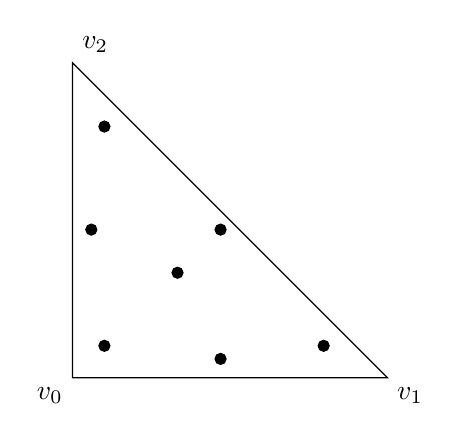
\begin{tikzpicture}[scale = 4,
]
	\def \xOneRef {0};
	\def \yOneRef {0};
	\def \xTwoRef {1};
	\def \yTwoRef {0};
	\def \xThreeRef {0};
	\def \yThreeRef {1};

	\coordinate (POneRef) at (\xOneRef, \yOneRef);
	\coordinate (PTwoRef) at (\xTwoRef, \yTwoRef);
	\coordinate (PThreeRef) at (\xThreeRef, \yThreeRef);


	\draw (0,0) -- (0,1) -- (1,0) -- cycle;

%draw point in ref triangle
	\draw[fill] (POneRef) circle (0.0pt) node [below left] {$v_0$};
	\draw[fill] (PTwoRef) circle (0.0pt)node [below right] {$v_1$};
	\draw[fill] (PThreeRef) circle (0.0pt)node [above right] {$v_2$};

	\def \a {0.470142};
	\def \b {0.0597159};
	\def \c {0.101287};
	\def \d {0.797427};
  	\draw[fill] \baryc {0.333333} {0.33333} {0.33333} circle (0.5pt);
  	\draw[fill] \baryc {\b} {\a} {\a} circle (0.5pt);
  	\draw[fill] \baryc {\a} {\b} {\a} circle (0.5pt);
 	\draw[fill] \baryc {\a} {\a} {\b} circle (0.5pt);
  	\draw[fill] \baryc {\d} {\c} {\c} circle (0.5pt);
  	\draw[fill] \baryc {\c} {\d} {\c} circle (0.5pt);
  	\draw[fill] \baryc {\c} {\c} {\d} circle (0.5pt);
\end{tikzpicture}
	\caption{Quadrature points for a integral over a triangle domain with $N=7$}
	 \label{fig: quadrature}
\end{figure}
Quadrature formulas, i.e. quadrature points and weights, especially for handling volume integrals can be found in \cite{Strout1971}.
To assemble the stiffness matrix $M$ the data we have to provide reduces to the functions values at the element or face quadrature points, respectively.  
In the SIPG method we to evaluate the bilinear form and the functional in \eqref{eq: DG system} for every combination of test functions. This means, at an element quadrature point we require the gradients, whereas at a face quadrature point we need information about the function values $u$ and the normal derivatives, i.e. $\nabla u \cdot \mathbf{n}$ of all test functions.

\subsection{A Reference Cell} \label{subsec: ref cell}
To reduce the storage space one usually specifies a \emph{reference cell} $T_{ref}$: We aim to relate triangles attributes to the reference cell attributes. There is for each triangle $T \in \triang$ an affine transformation $\Phi_T:T_{ref} \rightarrow T$ such that $\Phi_T$ maps $T_ref$ into $T$ and $\Phi$ maps the nodes of $T_ref$ onto the nodes of $T$.
%We make use of the triangle spanned by the points $(0,0)^t, (0,1)^t$ and $(1,0)^t$ for our reference cell. 
Since the DG spaces also allow discontinuous functions a basis $p^1_{ref},\dots,p^n_{ref}$ of $T_{ref}$ also induces a basis on every $T$ via $\Phi_T$, namely the basis consisting of 
\[
	p_T^i(x) := p^i_{ref}(\Phi_T^{-1}(x)), \qquad x \in T, 1 \leq i \leq n.
\]
The most famous basis polynomials are the Lagrange elements, i.e. given a set of points $P$ each Lagrange basis element evaluate at exactly one point of $P$ to one and vanishes at every other point of $P$. Due to this property this basis is also referred as a nodal basis. 
A huge benefit of the Lagrange elements are they form a interpolatory basis, i.e. the coefficients of a polynomial in Lagrange representation are the function values at the points of $P$.

Now most of the required data on a triangle $T$ can be easily derived knowing $\Phi_T$ and the reference cell $T_{ref}$. We explain how to do that in detail for the two-dimensional case.

\begin{example}\label{ex: base cell trafo}
From now on we consider $\Omega \subset \R^2$ and we choose the reference triangle to be the standard simplex, which is the triangle spanned by the points $\point 0 0, \point 0 1$ and $\point 1 0$.
Suppose we want to figure out the transformation for the triangle $T = \langle v_0,v_1,v_2 \rangle$.
It has to hold
\[
\Phi_T\left(\point 0 0\right) = v_0, \Phi_T\left(\point 0 1\right) = v_1 \textnormal{ and } \Phi_T\left(\point 1 0\right) = v_2.
\]
Since every two-dimensional affine transformation can be written in the form $\Phi(x) = Ax+b$ for some $A \in \R^{2 \times 2}$ and $b \in \R^2$ it is easy to verify that we have $A = \begin{pmatrix} v_1-v_0 & v_2-v_0\end{pmatrix}$ and $b = v_0$.
Having determined the transformation we are able to calculate its inverse $\Phi_T^{-1}(x) = A^{-1} (x-b) =: A^{-1} x- \tilde b$.
Combining the reference cell concept with barycentric coordinates we gain a connection between original and reference triangle. Let $\beta_0, \beta_1$ and $\beta_2$ be the barycentric coordinates of $x \in T$. We find
\begin{align*}
	p^i_T(x) =& p_T^i( \beta_0 v_0 +\beta_1 v_1 + \beta_2 v_2  ) \\
	=& p^i_{ref}(\Phi_T^{-1}(\beta_0 v_0 +\beta_1 v_1 + \beta_2 v_2)) \\
	=& p^i_{ref}(A^{-1}(\beta_0 v_0 +\beta_1 v_1 + \beta_2 v_2)- \tilde b)
\end{align*}
We recall that for barycentric coordinates $\sum_{i=0}^2 \beta_i = 1$ is valid and thus,
\begin{align*}
	p^i_T(x)
	=& p^i_{ref}(\beta_0(A^{-1}v_0 -\tilde b) +\beta_1(A^{-1}v_1 -\tilde b) + \beta_2(A^{-1}v_2 -\tilde b))\\
	=& p^i_{ref}(\beta_0 \Phi_T^{-1}(v_0) +\beta_1 \Phi_T^{-1}(v_1) + \beta_2 \Phi_T^{-1}(v_2)) \\
	=& p^i_{ref}(\beta_0 \point 0 0 +\beta_1 \point 0 1 + \beta_2 \point 1 0 ), \qquad 1 \leq i \leq n.
\end{align*}
Thus, basis function values in $T$ can be simply determined using barycentric coordinates. Henceforth we refer with $x_{ref}$  to the point $\beta_0 \point 0 0 +\beta_1 \point 0 1 + \beta_2 \point 1 0$ which is the to $x$ corresponding point in the reference triangle. In Figure \ref{fig: transformation} the connection between $x_{ref}$ and $x$ is shown.

\begin{figure}[H]
	
\usetikzlibrary{calc}
\usetikzlibrary{decorations.markings}
%\newcommand\fOne[2]{2*#1 + 0* #2 + 2}

%\fOne 1 1 

\begin{tikzpicture}[scale = 4,
]
	\def \xOneRef {0};
	\def \yOneRef {0};
	\def \xTwoRef {1};
	\def \yTwoRef {0};
	\def \xThreeRef {0};
	\def \yThreeRef {1};

	\coordinate (POneRef) at (\xOneRef, \yOneRef);
	\coordinate (PTwoRef) at (\xTwoRef, \yTwoRef);
	\coordinate (PThreeRef) at (\xThreeRef, \yThreeRef);

	\def \xRef {0.6};
	\def \yRef {0.2};
	\coordinate (PRef) at (\xRef, \yRef);


	\def \a {1.1};
	\def \b {0.4};
	\def \c {1.2};
	\def \d {0.3};

	\def \e {1.5};
	\def \f {0.5};

	\coordinate (xOneT) at ($({\a*\xOneRef+\b*\yOneRef+\e},{\c*\yOneRef+\d*\xOneRef+\f})$);
	\coordinate (xTwoT) at ($({\a*\xTwoRef+\b*\yTwoRef+\e},{\c*\yTwoRef+\d*\xTwoRef+\f})$);
	\coordinate (xThreeT) at ($({\a*\xThreeRef+\b*\yThreeRef+\e},{\c*\yThreeRef+\d*\xThreeRef+\f})$);

	\coordinate (xT) at ($({\a*\xRef+\b*\yRef+\e},{\c*\yRef+\d*\xRef+\f})$);


	\draw (0,0) -- (0,1) -- (1,0) -- cycle;
	\draw (xOneT) -- (xTwoT) -- (xThreeT) -- cycle;

%draw point in ref triangle
	\draw[fill] (POneRef) circle (0.6pt) node [below left] {$v^{ref}_0$};
	\draw[fill] (PTwoRef) circle (0.6pt)node [below right] {$v^{ref}_1$};
	\draw[fill] (PThreeRef) circle (0.6pt)node [above right] {$v^{ref}_2$};

	\draw[fill] (PRef) circle (0.6pt) node [left] {$x^{ref}$};


	\draw[fill] (xOneT) circle (0.6pt) node [left=0.1cm] {$v_0$};
	\draw[fill] (xTwoT) circle (0.6pt) node [right=0.2cm] {$v_1$};
	\draw[fill] (xThreeT) circle (0.6pt) node [above right] {$v_2$};

	\draw[fill] (xT) circle (0.6pt) node [left=0.1cm] {$\Phi(x^{ref}) =x$};

%	\draw[->, shorten >=0.5cm, shorten <=1cm] (PRef) edge [bend right] ($(xT)$);

	\draw[
			decoration = {markings, mark=at position 0.98 with {\arrow[scale=3, black]{stealth}}},
			postaction = {decorate},
			shorten >=5,
			shorten <=5,
			bend right] (PRef) to node [below] {{\Large $\Phi$}} ($(xT)-(0.005,0.005)$) ;

	%draw axes
	\draw[thick,->] (0, 0) -- (1.3,0);
	\draw[thick,->] (0, 0) -- (0,1.3);
	


\end{tikzpicture}
	\caption{Transformation of reference cell}
	 \label{fig: transformation}
\end{figure}

Similarly we can affiliate the determination of the gradient in $T$ to a calculation in $T_{ref}$. With the chain rule we have
\begin{align*}
	\left(\nabla_x p_T^i(x)\right)^t = D_x p_T^i(x) =& D_x p^i_{ref}(\Phi_T^{-1}(x)) \\
	  =& D_{\Phi_T^{-1}(x)}p^i_{ref}(\Phi_T^{-1}(x)) \cdot D_x  \Phi_T^{-1}(x) \\
	  =& D_{x_{ref}}p^i_{ref}(x_{ref}) \cdot  A^{-1}
\end{align*}
and thus
\begin{align}
	\nabla_x p_T^i(x) = A^{-t} \cdot \nabla_{x_{ref}}(x_{ref}), \qquad 1 \leq i \leq n. \label{eq: ref gradient}
\end{align}

Analogous proceeding yields for the Hessian matrix
\begin{align}
D_x^2p_T^i(x) = A^{-t} D_{x_{ref}}^2p^i_{ref}(x_{ref})  A^{-1}, \qquad 1 \leq i \leq n.
\end{align}

Concluding, if we need to determine function values, gradient and Hessian of a basis function on a cell, we only need the Jacobian of its transformation, i.e. $A$. We are able to calculate all further information with the data provided by the reference triangle.
\end{example}

\subsection{Refinement and Base Cells}\label{subsec: refinement and base cells}
In the rest of this section let us assume we have a fixed triangulation of a two-dimensional domain $\Omega$. 
Suppose the mesh of our triangulation is created by refinement of a coarser mesh. We choose a specific kind of uniform refinement: Given a triangulation $\triang$ every triangle $T \in \triang$ is divided into four congruent triangles as is shown in Figure \ref{pic: refinement}. We note that the diameter of each triangles in the finer grid is halved and therefore we denote the finer grid by $\triangFine$. %Additionally the small triangles inherit the same angles as the original cell as we verify with the intercept theorem.

\begin{figure}[h]
\usetikzlibrary{calc}

		\begin{center}
		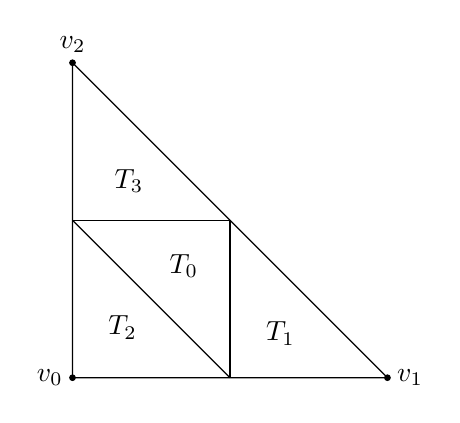
\begin{tikzpicture}
%define coordinates
			\coordinate (vEins) at (0,0) ;
			\coordinate (vZwei) at (0:4cm);
			\coordinate (vDrei) at (90:4cm);

%draw triangle
			\draw (vEins) -- (vZwei) -- (vDrei) -- cycle;

%draw refined triangle
			\draw ($(vEins)!0.5!(vZwei)$) -- ($(vEins)!0.5!(vDrei)$);
			\draw ($(vDrei)!0.5!(vZwei)$) -- ($(vEins)!0.5!(vDrei)$);
			\draw ($(vEins)!0.5!(vZwei)$) -- ($(vZwei)!0.5!(vDrei)$);

%draw nodes
			\draw[fill =black] (vEins) circle (1pt) node[left] {$ v_0$};
			\draw[fill =black] (vZwei) circle (1pt) node[right] {$v_1$};
			\draw[fill =black] (vDrei) circle (1pt) node[above] {$v_2$};

%			\draw node at (30:2.4cm) {$T_1$};

			\draw node at (45:0.9cm) {$T_2$};
			\draw node at (45:2cm) {$T_0$};
			\draw node at (74:2.6cm) {$T_3$};
			\draw node at (12:2.7cm) {$T_1$};

		\end{tikzpicture}
		\end{center}

\caption{Refinement of a triangle}
 \label{pic: refinement}
\end{figure}

We associate the new refined triangles with the original cell which we call their \emph{base cells} $B$. Repeating the refinement we can always relate a cell in the finest mesh with a base cell in the original triangulation. We can find an affine mapping $\Psi_T:B \rightarrow T$ transforming the base cell $B$ to $T$ such that $\Phi_T = \Psi_T \circ \Phi_B$. This implies also that for the Jacobians $A_{\Phi_T}, A_{\Psi_T}, A_{\Phi_B}$ of the affine transformations $\Phi_T, \Psi_T,\Phi_B$ holds
\begin{align}
A_{\Phi_T}=A_{\Psi_T} A_{\Phi_B}
\end{align} 

This makes saving information about the base cell very beneficial for the transformation matrix $A_{\Psi_T}$ is a diagonal matrix which even has the same entries along the diagonal. It even follows that basis function data on two triangles with the same base cell only differ in a constant factor. Yet another benefit of the relation between cells and their base cells is they have the same, or for the innermost triangle ($T_0$ in figure \ref{pic: refinement}) opposite directed, normals.

\begin{example}\label{ex: leaf cell trafo}
In the two-dimensional case the Jacobian $A_{\Psi_T}$ of a transformation $\Psi_T$ from the base cell $B$ to a $l$ times refined triangle $T$ is $
	\begin{pmatrix}
		\frac 1 {2^l} & 0 \\ 0 & \frac 1 {2^l}
	\end{pmatrix} \text{ or }
	\begin{pmatrix}
		-\frac 1 {2^l} & 0 \\ 0 & -\frac 1 {2^l}
	\end{pmatrix}$, respectively if the number of intermediate base cells being an inner triangle during refinement  has been odd.

 To a point $x \in T$ we can determine a corresponding base cell point $x_B$, namely the point which satisfies $x = \Psi_T(x_B)$. With the help of \eqref{eq: ref gradient} we find the identity
\begin{align}
\nabla_x p_T^i(x) &= A_{\Phi_T}^{-t} \nabla_{x_{ref}} p^i_{ref} (x_{ref}) \nonumber\\
 &= A_{\Psi_T}^{-t} A_{\Phi_B}^{-t} \nabla_{x_{ref}} p^i_{ref} (x_{ref}) \nonumber\\
&= \epsilon 2^l A_{\Phi_B}^{-t} \nabla_{x_{ref}} p^i_{ref}(x_{ref}), \qquad \epsilon \in \{+,-\} \label{eq: trafo grad},
\end{align}
with $l \in \N$ indicating how often $T$ is refined with respect to the original mesh.\\
Analogously we have
\begin{align}
\nabla_x p^i(x) \mathbf n &= 2^l  A_{\Phi_B}^{-t} \cdot \nabla_{ref}p^i_{ref}(x_{ref}) \mathbf{ n_{b}} \qquad \text{ and } \label{eq: trafo normal der} \\
D_x^2 p^i(x) &= 2^{2l}  A_{\Phi_B}^{-t} D_{x_{ref}}^2 p^i_{ref}(x_{ref}), \qquad 1 \leq i \leq n,
\end{align}
where $\mathbf n_b$ is the to $n$ corresponding normal in the base cell. Note, that \eqref{eq: trafo normal der} even holds for inner refined triangles: The minus sign of the gradient cancels with the minus sign of the base cell normal $n_B$ since $n_B$ is opposite directed as the corresponding normal $n$ of a inner triangle.\\
Another case where the sign of the gradient \eqref{eq: trafo grad} could be important when we evaluate of the first part of the bilinear form, i.e. $\nabla \phi \cdot A \nabla v$. We first note, that two basis functions $p_T^i$ and $p_T^j$ having only support on $T$ are created with the same affine mapping $\Phi_T$. Hence they have the same transposed, inversed Jacobian $A^{-t}_{\Phi_T}=\epsilon 2^l A_{\Phi_b}^{-t}$ and therefore the sign on the right-hand side in \eqref{eq: trafo grad} is for both gradients the same. Because we multiply both gradients a sign change between base and the actual cell does not affect the evaluation of our bilinear form. 
Of course for other combinations of basis polynomials the latter volume integral always equals zero because the polynomials' support is chosen in such a way that all other gradients vanish in the interior of $T$.

A usual source of errors are the signs of the terms
\[
	\jump {v \average{ A \nabla w }} = v^+ \frac 1 2  \left(A^+ \nabla w^+ + A^- \nabla w^-\right) \cdot \mathbf n^+ + v^- \frac 1 2 \left(A^+ \nabla w^+ + A^- \nabla w^-\right) \cdot \mathbf n^-.
\]
Since for two adjacent triangles always $\mathbf n^+ = - \mathbf n^-$ holds, we also have $A^+ \nabla w^+ \mathbf n^-= -A^+ \nabla w^+ \mathbf n^+$ and $A^- \nabla w^- \mathbf n^+= -A^- \nabla w^- \mathbf n^-$. Hence we can calculate the expression using \eqref{eq: trafo normal der}. Note that all basic functions have support on only one triangle, such that for a evaluation of a basic functions $v_B$ either $v_B^+$ or $v_B^-$, just as for a basic functions $w_B$ either $w_B^+$ or $w_B^-$ equals to zero.

So, we are able to save a lot of memory if we store instead of all data at every quadrature points in each refined cell just the data of the base cell and the number of refinements. The refined cells contained in the actual mesh are referred to as \emph{leaf cells}.
\end{example}

\subsection{Assembly Loop}\label{subsec: assembly loop}
Another crux of the implementation is the handling of face terms, let us be more specific: We mentioned earlier that we evaluate the bilinear form cell-wise. Hence the volume integrals are calculated visiting every cell only once. Let us now consider when do we compute the edge integrals.\\
\begin{algorithm}[H]
\caption{An assembling loop for a DG method}
\label{alg: assembling}
\begin{algorithmic}
\Ensure every cell flag is false
\For {cell in all leaf cells}  
\State get cell data
\State assemble volume integrals 
	\For {face in faces(cell)}
		\If {neighbour across the face exists} 
			\If {neighbour flag not set}
					\State get neighbour cell data
					\State assemble face terms
			\EndIf
		\Else
			\State assemble boundary terms
		\EndIf
\EndFor
	\State cell flag to true 
\EndFor
\State Reset every cell flag to false
\end{algorithmic}
\end{algorithm}
Face terms can be assembled in two simple or a single more complex step.
For the two-step variant the face terms are split up into the contributions of their two adjacent cells, such that the first part is assembled when processing the first to the edge adjacent cell and the second during the processing of the other adjacent cell. \\
In the one step variant we handle a face term when visiting an adjacent cell for the first time. To detect the first time we introduce a flag for every leaf cell indicating whether the cell has been processed yet. Now, each time the assembling algorithm visits a face it determines the neighbouring cell and checks if the face has already been processed. 

Algorithm \ref{alg: assembling} from \cite{BMV2009} illustrates how to perform this one step approach. 
The advantage of this approach that it can be easily extended to the case of a non-uniform refinement, i.e. adjacent base cells are not necessarily refined equally often, and different kinds of cell types.

In \cite{BMV2009} Brix et alt. also develop a data structure efficiently handling all the mentioned requirements among a lot of other features. The implementation used for the Numerical Results in Section \ref{sec: numerical results our Method} is based on this data structure.

After we saw the main implementation points of a DG method we need some algebraic and analytic identities for the Hessian matrix to develop a DG method handling the \MA equation.
\section{Hessian Identities}

We begin with the notion of the cofactor matrix which is later important for the linearisation of the \MA equation.
\begin{definition}[Cofactor Matrix] \label{def: cof matrix}
	The \emph{cofactor matrix} of a matrix $A \in \R^{d \times d}$ is defined by the entries
	\begin{align}
	(\mycof A )_{i,j} := (-1)^{i+j} \mydet{A_{ij}},
	\end{align}
	where $A_{ij}$ denotes the matrix resulting from deleting the $i$-th row and $j$-column in $A$.
\end{definition}

We observe that in the two-dimensional case the cofactor matrix of the Hessian simplifies to
\begin{align}
\mycof {D^2 u} = \begin{pmatrix}
								\dxx{x_2} u & -\frac {\partial }{\partial x_1 x_2} u\\
								-\frac {\partial }{\partial x_2 x_1} u & \dxx{x_1} u
							\end{pmatrix}.
\end{align}

\begin{definition}[Frobenius Product] \label{def: frobenius product}
	The \emph{Frobenius product} : of two matrices $A, B \in \R^{d \times d}$ is defined by
	\[
		A:B := \sum_{1 = i,j} ^d a_{i,j} b_{i,j}.
	\]
\end{definition}

Very helpful is the relation between the determinant and the cofactor matrix.
\begin{lemma}\label{la: rel det cofactor}
	For every matrix $A  \in \R^{d \times d}$ it holds
	\[
		d \mydet A = \mycof A: A.
	\]
\end{lemma}
\begin{proof}
	By Laplace's formula it holds for any $1 \leq j \leq d$
	\[
		\mydet A = \sum\limits_{i = 1}^{d} a_{i,j} (\mycof A )_{i,j}.
	\]
	Summing over all $j$ yields
	\[
		d \mydet A = \sum\limits_{j= 1}^{d} \sum\limits_{i = 1}^{d} (\mycof A )_{i,j}  a_{i,j}  = \mycof A: A.
	\]
	\phantom{blub}
\end{proof}

Another advantage is the behaviour of the cofactor matrix of a Hessian if a divergence is applied to it:
\begin{definition}[Matrix Divergence]
The divergence $\nabla \cdot A$ for a matrix $A$ is defined by taking the divergence row-wise, i.e.
\[
	\nabla \cdot A := \begin{pmatrix} \nabla \cdot A_1 \\ \vdots \\ \nabla \cdot A_d\end{pmatrix}
	= \begin{pmatrix} \sum_{j = 1}^{d} \dx{x_j} a_{1,j} \\ \vdots \\ \sum_{j = 1}^{d} \dx{x_j} a_{d,j}\end{pmatrix}.
\]
where $A_i$ denotes the $i$-th row of $A$.
	
\end{definition}

\begin{lemma}[Divergence-Free Property of Cofactor Matrices] \label{la: divergence free cof}
For smooth functions $u:\Omega \rightarrow \R$ with $\Omega \subset \R^2$ the cofactor matrix of the Hessian is divergence-free, i.e.
\[
	\nabla \cdot \mycof{D^2 u} = 0.
\] 
\end{lemma}
\begin{proof}
It holds that
\begin{align*}
	\nabla \cdot \mycof{D^2 u} = \sum_{i=1}^{2} \dx{ x_i}\mycof{D^2 u}_i = 
	\begin{pmatrix}
		\frac {\partial^3} {\partial x_1 {x_2}^2 } u -\frac {\partial^3} {\partial{x_2} x_1 {x_2}} u\\
				\frac {\partial^3} {\partial {x_1}x_2 {x_1}} u-\frac {\partial^3} {\partial x_2 {x_1}^2 } u
	\end{pmatrix}.
\end{align*}
By Schwarz' theorem the latter equals zero if $u$ is twice continuous differentiable.
\end{proof}

The divergence-free property yields to an integration by parts rule.
\begin{lemma}[Integration by parts for the Frobenius product] \label{la: integration by parts Frobenius}
For a Frobenius product with the Hessian's cofactor matrix  the following integration by parts rule holds for smooth $u$ and any $B \in [H^1(\Omega)]^{2 \times 2}$
\[
	\myIntX  \Omega { (D^2 u : B)} = 
		- \myIntX  \Omega { (\nabla \cdot B) \cdot \nabla u }
		+ \myIntS  {\partial \Omega} {  B \nabla u \;\bf n}.
\] 
\end{lemma}

\begin{proof}
The proof is based on applying integration by parts row-wise. Hence, we have
\begin{align*}
- \myIntX  \Omega { (\nabla \cdot B) \cdot \nabla u} &= 
- \myIntX  \Omega { \sum_{i = 1}^{d} (\nabla \cdot B_i) \dx {x_i} u} \\
&=  \myIntX  \Omega { \sum_{i = 1}^{d} B_i \cdot  (\nabla \dx {x_i} u)} 
	- \myIntS  {\partial \Omega} { \sum_{i = 1}^{d} (B_i) \dx {x_i} u \;\mathbf{n}} \\
&=  \myIntX  \Omega { \sum_{i = 1}^{d}\sum_{j= 1}^{d} B_{ij} \dxy {x_i}{x_j} u}
	- \myIntS  {\partial \Omega} { B \nabla u \;\mathbf{n}} \\
&=  \myIntX  \Omega { (D^2 u : B)}
	- \myIntS  {\partial \Omega} { B \nabla u \;\mathbf{n} }.
\end{align*}
\end{proof}

In future talking about weak formulations it is handy to have a divergence form of the latter Frobenius product.
\begin{lemma}[Divergence form of the Frobenius Product] \label{la: An application of the divergernce product rule}
For smooth $u:\Omega \rightarrow \R$ with $\Omega \subset \R$ and $v\in H^2(\Omega)$, there holds
\[
		\nabla \cdot \left( \mycof {D^2 u } \nabla v \right) %- \nabla \cdot \left(\mycof {D^2 u }\right) \nabla v
		= \mycof {D^2 u}: D^2 v.
\] 
\end{lemma}

\begin{proof}
By the definition of the divergence and the product rule we obtain
\begin{align*}
\nabla \cdot \left( \mycof {D^2 u } \nabla v \right) =&%- \nabla \cdot \left(\mycof {D^2 u }\right) \nabla =& 
\sum_{i= 1}^{d} \dx {x_i} 	\left( \sum_{j= 1}^{d} \mycof {D^2 u }_{i,j} \dx{x_j} v \right)\\
%&-  \sum_{j= 1}^{d}  \sum_{i= 1}^{d} \left(\dx {x_i} \mycof {D^2 u }_{i,j}  \right) \dx{x_j} v \\
=&  \sum_{i= 1}^{d} \sum_{j= 1}^{d}  \left(\dx {x_i} \mycof {D^2 u }_{i,j}  \right) \dx{x_j}v + \sum_{i= 1}^{d} \sum_{j= 1}^{d}  \mycof {D^2 u }_{i,j} \dxy{x_j}{x_i}v\\
=&  \sum_{j= 1}^{d}  \nabla \cdot \left(\mycof {D^2 u }\right)_j \dx{x_j}v + \sum_{i= 1}^{d} \sum_{j= 1}^{d}  \mycof {D^2 u }_{i,j} \dxy{x_j}{x_i}v\\
=&   \nabla \cdot \left(\mycof {D^2 u }\right) \nabla v+ \mycof {D^2 u }:D^2v.
\end{align*}
The statement results from the fact that the cofactor matrix of the Hessian is divergence-free.
\end{proof}
